% Vorlage fuer latex-beamer-Praesentationen unter Verwendung des Corporate 
% Designs der Uni.
%
% Basiert auf der alten Vorlage von Carsten Bockelmann 
% (bockelmann@ant.uni-bremen.de), angepasst an das Corporate Design von 
% Henning Paul (paul@ant.uni-bremen.de) unter Verwendung der Vorlage von
% Dirk Lorenz und Kristan Bredies aus dem Zentrum fuer Technomathematik
% ({dlorenz,kbredies}@math.uni-bremen.de)

\documentclass[10pt]{beamer}

\mode<presentation>
{
  % Das ANT-Theme benutzen
  % Titel in Kopfzeile, kleine Navigationselemente, Seitennummer anzeigen,
  % Autor dauerhaft eingeblendet lassen
  % \usetheme[headlinetitle,navline=small,footlinenumber,footlineauthor]{ANT}

  % Autor nicht dauerhaft einblenden
   \usetheme[headlinetitle,navline=small,footlinenumber]{Bremen}

  %
  % Die vollstaendige Dokumentation zu unserem Theme findet sich in der Datei 
  % beamerZeTeMdoc.pdf, da es auf dem Theme der Technomathematiker aus dem 
  % ZeTeM basiert.
  %
  % Es koennen bis zu zwei zusaetzliche Logos (zu unserer Ameise oben links
  % und dem Uni-Logo unten links) hinzugefuegt werden, diese erscheinen dann
  % rechts neben dem Uni-Logo.
  % \partnerlogo{
	% \includegraphics[height=2.6\baselineskip]{TZI.pdf}}
  % \secondarypartnerlogo{
	% \includegraphics[height=2.6\baselineskip]{DFG_zweizeilig_blau.pdf}}

  % Dieses sind Standard-latex-beamer-Optionen:
  %
  % Der mathematische Schriftsatz ist mit Serifen
  \usefonttheme[onlymath]{serif}
  % Noch nicht aufgedeckte Punkte erscheinen ausgegraut
  \setbeamercovered{transparent}
  % Bild-/Tabellenueberschriften sind sehr klein
  \setbeamerfont{caption}{size=\tiny}

}



%\usepackage[german]{babel}
% oder was auch immer

\usepackage[utf8]{inputenc}
% oder was auch immer

\usepackage{color,soul}
\definecolor{darkblue}{rgb}{0,0,0.5}
\setulcolor{darkblue}

\usepackage{hyperref}
\hypersetup{
    pdftitle={},
    pdfsubject={},
    pdfauthor={Sadik Özoguz},
    pdfkeywords={},
    % pdfpagemode=None, %deprecated
    plainpages=false,
    pdfstartview=Fit,
    breaklinks=true,
    colorlinks=false,
    pdfhighlight=/N,
    % define colors, even if not used
    linkcolor=blue,
    citecolor=blue,
    urlcolor=blue,
    citebordercolor=1 1 1,
    filebordercolor=1 1 1,
    linkbordercolor=1 1 1,
    menubordercolor=1 1 1,
    % pagebordercolor=1 1 1, %deprecated
    urlbordercolor=1 1 1,
    % pdfborder=1 1 1 %erzeugt fehler im footer
  }

\title{Eigenschaftsorientiertes Testen sicherheitskritischer Systeme}
\author{Sadik Özoguz}
\institute{Universit{\"a}t Bremen}
\date[29.11.2018]{29. November 2018}

\newcommand{\W}{\mathcal{W}}
\newcommand{\F}{\mathcal{F}}

\subject{Presentation}
%\AtBeginSection[]
%{
%  \begin{frame}
%    \tableofcontents[currentsection]
%  \end{frame}
%}

% Hier beginnt der redaktionelle Inhalt
\usepackage[style=alphabetic]{biblatex}

\bibliography{literatur.bib}

\usepackage{color, colortbl}
\usepackage{pgfplots}
\usepackage{pgfplotstable}
\usepackage{subcaption}
\usepackage[ngerman]{babel}
\addto{\captionsngerman}{%
  \renewcommand*{\contentsname}{Inhalt}
  \renewcommand*{\listfigurename}{Abbildungen}
  \renewcommand*{\listtablename}{Tabellen}
  \renewcommand*{\figurename}{Abb.}
  \renewcommand*{\tablename}{Tab.}
}

\newcommand{\pref}{\text{\rm Pref}}
\newcommand{\successor}{\text{\rm Succ}}
\newcommand{\after}{\text{\rm -\underline{after}-}}
\newcommand{\ii}[1]{\underline{#1}}
\newcommand{\fun}{\rightarrow}
\newcommand{\dist}{\text{\rm Dist}}
\newcommand{\equivs}{\text{\bf equiv}}
\newcommand{\ol}{\overline}
\newcommand{\pesnot}[2]{\mathrel{\widesimsnot{#2}{#1}}}
\newcommand{\pe}{\sim_s}
\newcommand{\pes}[2]{\mathrel{\widesims{#2}{#1}}}
\newcommand{\sims}[1]{\stackrel{#1}{\sim}}
\newcommand{\id}{\mathbf{id}}
\newcommand{\ps}{\le_s}
\newcommand{\pss}[1]{\stackrel{#1}{\ps}}
\newcommand{\primem}{\mathbf{prime}}
\newcommand{\TS}{{\text{TS}}}
\newcommand{\ist}{\mbox{{\tt true}}}
\newcommand{\isf}{\mbox{{\tt false}}}
\newcommand{\bzgl}{bzgl.\@\xspace}
\newcommand{\bzw}{bzw.\@\xspace}
\newcommand{\ca}{ca.\@\xspace}
\newcommand{\dah}{d.\thinspace{}h.\@\xspace}
\newcommand{\Dah}{D.\thinspace{}h.\@\xspace}
\newcommand{\ds}{d.\thinspace{}sind\@\xspace}
\newcommand{\evtl}{evtl.\@\xspace}
\newcommand{\ia}{i.\thinspace{}Allg.\@\xspace}
\newcommand{\sa}{s.\ auch\@\xspace}
\newcommand{\su}{s.\ unten\@\xspace}
\newcommand{\backupbegin}{
   \newcounter{finalframe}
   \setcounter{finalframe}{\value{framenumber}}
}
\newcommand{\backupend}{
   \setcounter{framenumber}{\value{finalframe}}
}

\usepackage[ruled]{algorithm2e}

\setbeamertemplate{section page}
{
    \begin{centering}
    \begin{beamercolorbox}[sep=12pt,center]{part title}
    \usebeamerfont{section title}\insertsection\par
    \end{beamercolorbox}
    \end{centering}
}

\begin{document}

\begin{frame}
  \titlepage
\end{frame}

\begin{frame}
  \tableofcontents
\end{frame}


\section{Einleitung}

\begin{frame}
  \frametitle{Motivation / Motivation}
  \begin{itemize}
    \item MBT: Modell $\rightarrow$ (vollständige) Test Suite
    \item Je größer die Test Suite, desto teurer das Testen
    \item<2-> Stattdessen: Nachweis einer Eigenschaft
    \item<3-> Ziel: Kleinere Testsuite, aber vollständig bezüglich dieser Eigenschaft
  \end{itemize}
\end{frame}
\section{DFSM}
\begin{frame}
  \frametitle{DFSM}

  \begin{definition}[Finite State Machine\footnote{Endlicher Zustandsautomat}]
    Eine Finite State Machine (FSM) ist ein 5-Tupel $$M=(Q,q_0,\Sigma_I,\Sigma_O,h)$$
    $Q$: Zustandsraum\\
    $q_0\in Q:$ Anfangszustand\\
    $\Sigma_I$, $\Sigma_O$ : Ein-, Ausgabealphabet\\
    $h \subseteq Q \times \Sigma_I \times \Sigma_O \times Q$ : Übergangsrelation 
  \end{definition}
  Deterministisch (DFSM): $(q,x,y_1,q_1),(q,x,y_2,q_2) \in h: (y_1 = y_2 \wedge q_1 = q_2)$
\end{frame}

\begin{frame}
\frametitle{FSM Eigenschaften}
\begin{itemize}
  \item Vollständig spezifiziert (\emph{completely specified})$$\forall q\in Q, x\in \Sigma_I : \exists y \in \Sigma_O, q'\in Q : (q,x,y,q')\in h$$
  \item Die Sprache eines Zustandes $q \in Q$ ist eine Menge von Eingabe-/Aus\-gabefolgen $$L(q)= \{\overline{x}/\overline{y} ~|~ \exists q' \in Q : (q,\overline{x}, \overline{y}, q') \in h \}$$
  \item I/O-äquivalent: $L(q_1) = L(q_2)$ bzw. $L(M_1) = L(M_2)$ $$q_1 \sim q_2, M_1 \sim M_2$$
  \item Minimal: Wenn keine zwei Zustände einer DFSM zueinander äquivalent sind, ist die DFSM \emph{minimal}.
\end{itemize}
\end{frame}
\section{$H$-Methode}
\begin{frame}
  \frametitle{Vergleich von Methoden}
  \begin{figure}
	  \caption{Quelle: \emph{A. T. Endo and A. Simao, "Experimental Comparison of Test Case Generation Methods for Finite State Machines," 2012 IEEE Fifth International Conference on Software Testing, Verification and Validation, Montreal, QC, 2012, pp. 549-558.} }
	  \centering
	  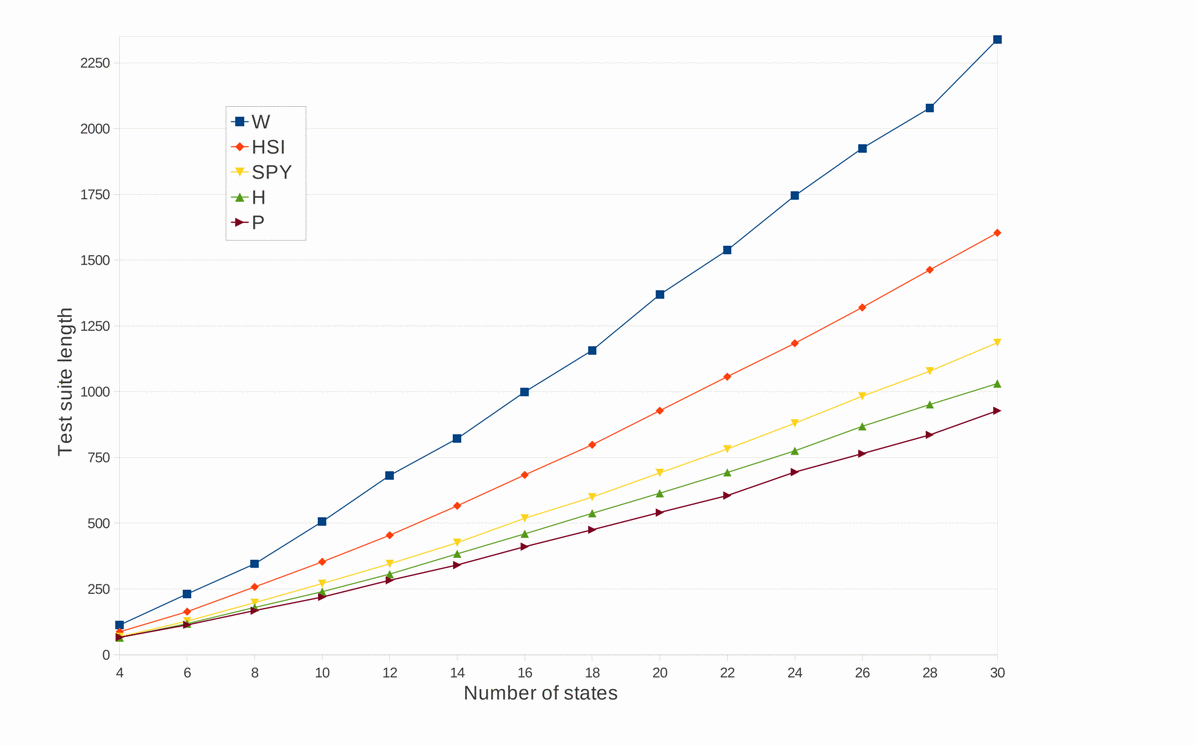
\includegraphics[width=0.85\textwidth]{images/methodComparison}
	\end{figure}

\end{frame}

\begin{frame}
  \frametitle{$H$-Methode}
  Gegeben seien eine vollständige, minimale DFSM mit einer Zustandsüberdeckung $V$ und $n$ Zuständen und~ein~Sicherheitsparameter~$m$ mit $m \geq n$.
  \begin{itemize}
    \item $A=V\times V$
  	\item $B=V\times (V.\bigcup\limits_{i=1}^{m-n+1}.\Sigma_I^i)$
  	\item $C=\{(\alpha,\beta)~|~\alpha,\beta\in V.\bigcup\limits_{i=1}^{m-n+1}.\Sigma_I^i, \alpha \in \text{Pref}(\beta)\}$
  \end{itemize}
  Für alle Paare $(\alpha, \beta) \in A\cup B \cup C$, falls $\delta(q_0,\alpha) \not \sim \delta(q_0,\beta)$, dann enthält die Test Suite $\alpha.\gamma,\beta.\gamma$. $\gamma$ ist die \emph{distinguishing trace} für $\delta(\alpha)$ und $\delta(\beta)$.
\end{frame}

\begin{frame}
\frametitle{$H$-Methode - Beispiel}
\begin{columns}[T] % align columns

\begin{column}{.4\textwidth}
\textbf{Liste von Paaren $(\alpha,\beta)$}\\
  \begin{itemize}
	\item<1>$V.\bigcup\limits_{i=1}^{m-n+1}.\Sigma_I^i$
	\item<2-3>\only<1-2>{$(aa,b)$}\only<3->{$(aa,b) \rightarrow a$}
    \item<4-5>\only<1-4>{$(aa,\epsilon)$}\only<5->{$(aa,\epsilon) \rightarrow b$}
    \item<6-7>\only<1-6>{$(ba,a)$}\only<7->{$(ba,a) \rightarrow a$}
    \item<8-9>\only<1-8>{$(ba,\epsilon)$}\only<9->{$(ba,\epsilon) \rightarrow a$}
    \item<10-11>\only<1-10>{$(ab,a)$}\only<11->{$(ab,a) \rightarrow a$}
    \item<12-13>\only<1-12>{$(bb,a)$}\only<13->{$(bb,a) \rightarrow b$}
  \end{itemize}
\end{column}%

\begin{column}{.70\textwidth}
\centering
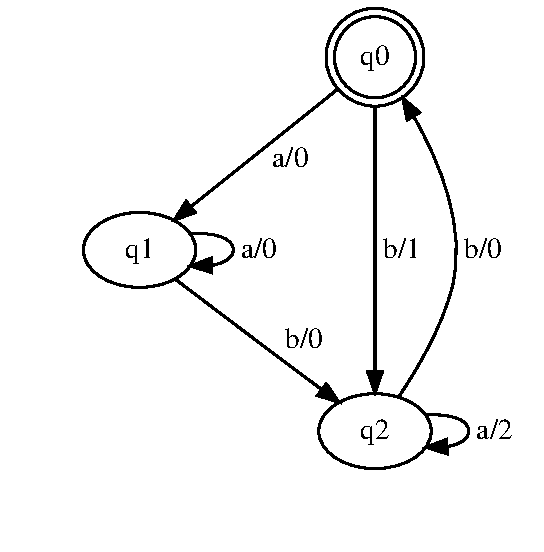
\includegraphics[width=0.5\textwidth]{images/fsm-example01_orig}%
\only<1-2>{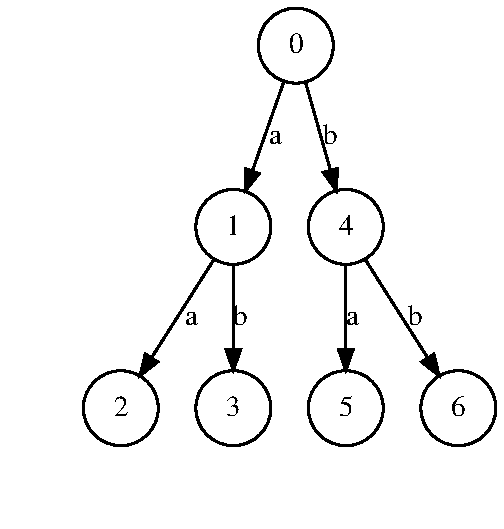
\includegraphics[width=0.5\textwidth]{images/HTree01}}%
\only<3>{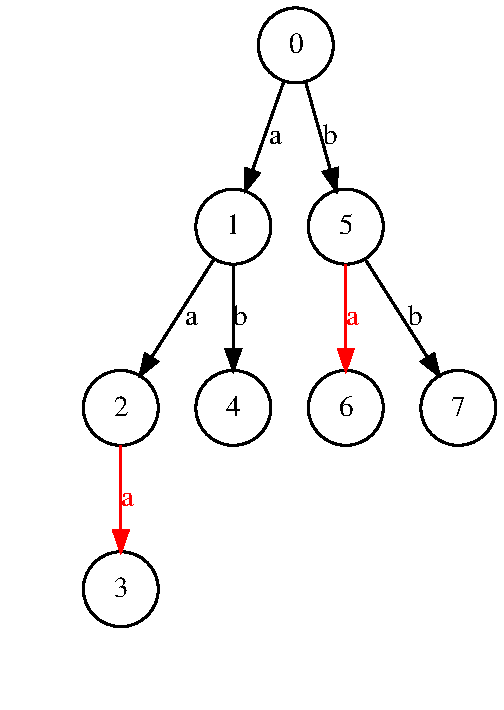
\includegraphics[width=0.5\textwidth]{images/HTree02_c}}%
\only<4>{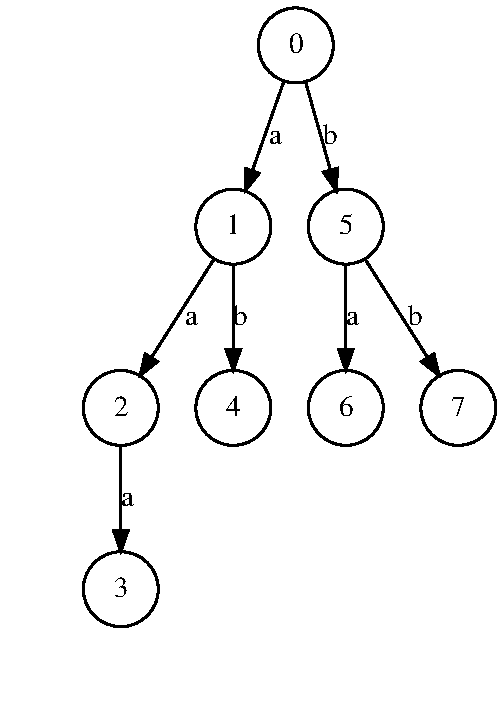
\includegraphics[width=0.5\textwidth]{images/HTree02}}%
\only<5>{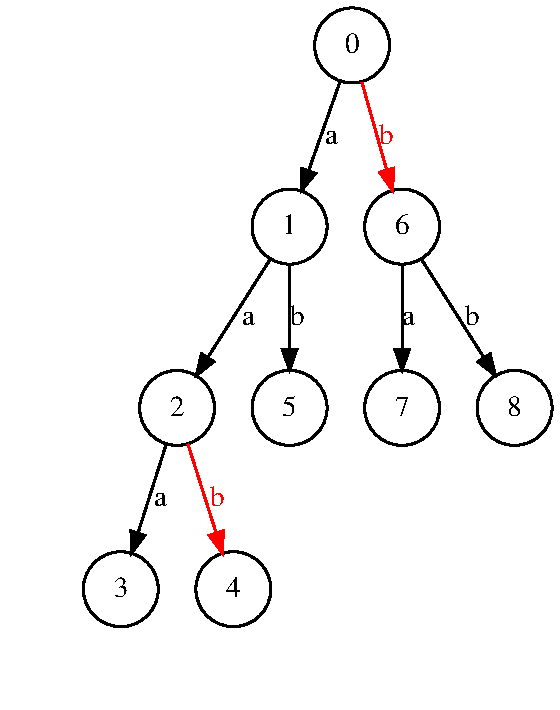
\includegraphics[height=0.6\textheight]{images/HTree03_c}}%
\only<6>{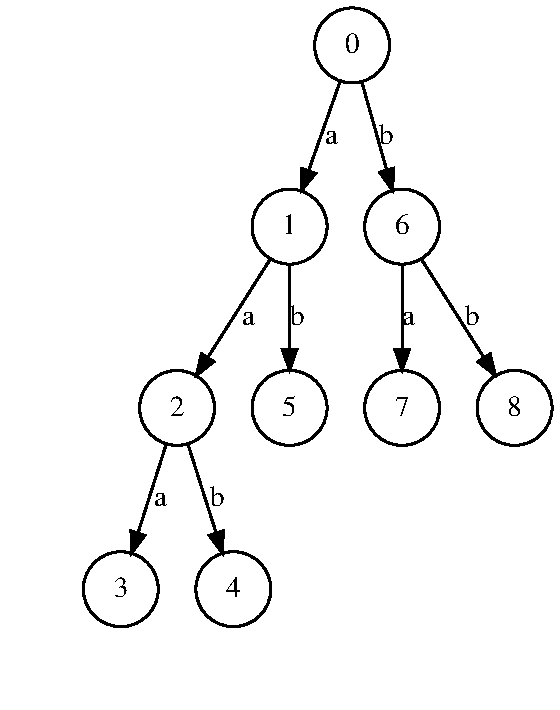
\includegraphics[height=0.6\textheight]{images/HTree03}}%
\only<7>{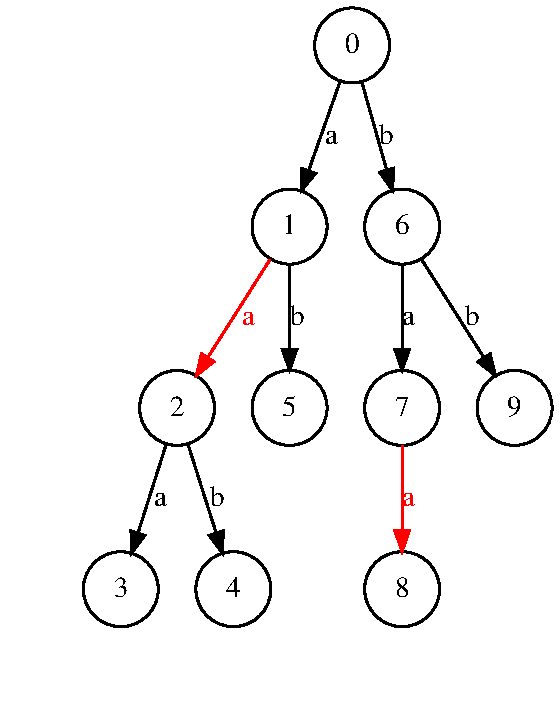
\includegraphics[height=0.6\textheight]{images/HTree04_c}}%
\only<8>{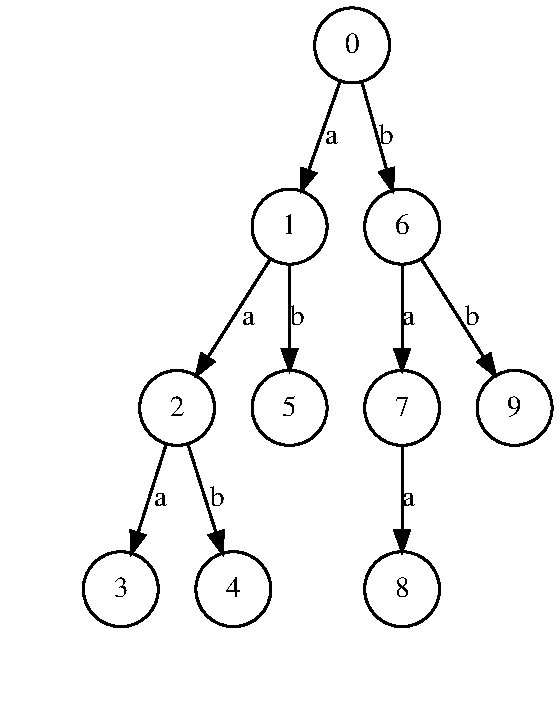
\includegraphics[height=0.6\textheight]{images/HTree04}}%
\only<9>{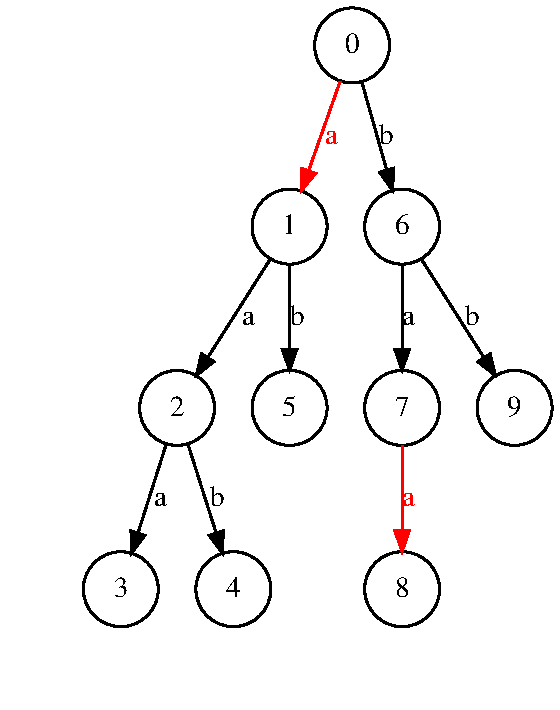
\includegraphics[height=0.6\textheight]{images/HTree05_c}}%
\only<10>{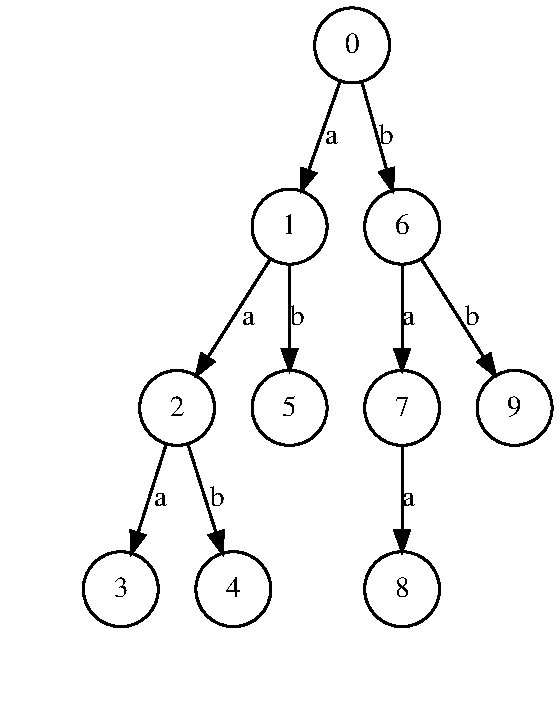
\includegraphics[height=0.6\textheight]{images/HTree05}}%
\only<11>{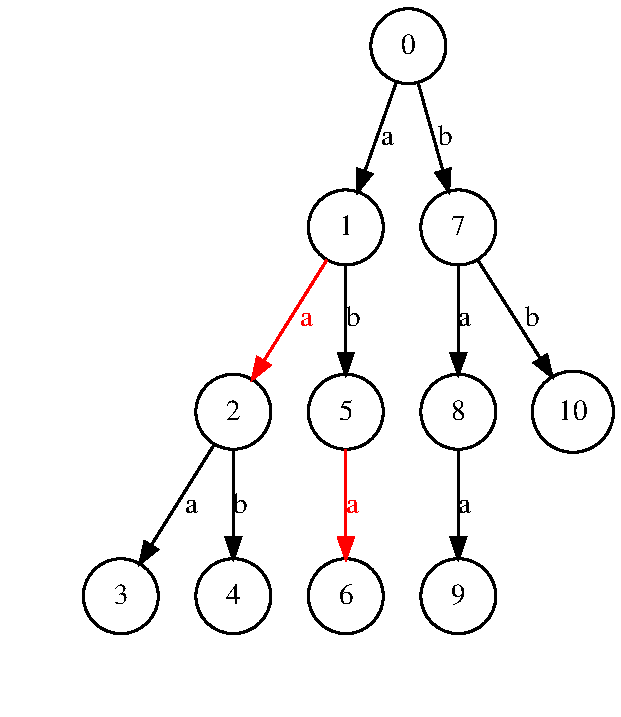
\includegraphics[height=0.6\textheight]{images/HTree06_c}}%
\only<12>{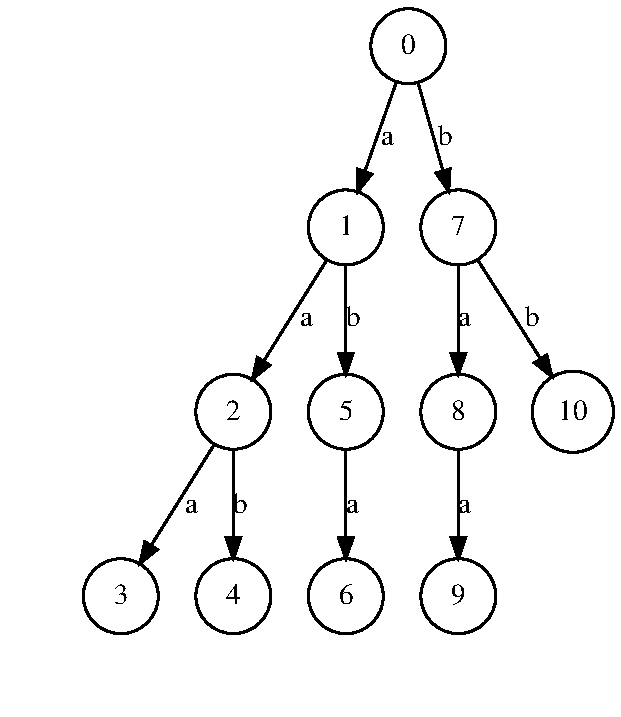
\includegraphics[height=0.6\textheight]{images/HTree06}}%
\only<13>{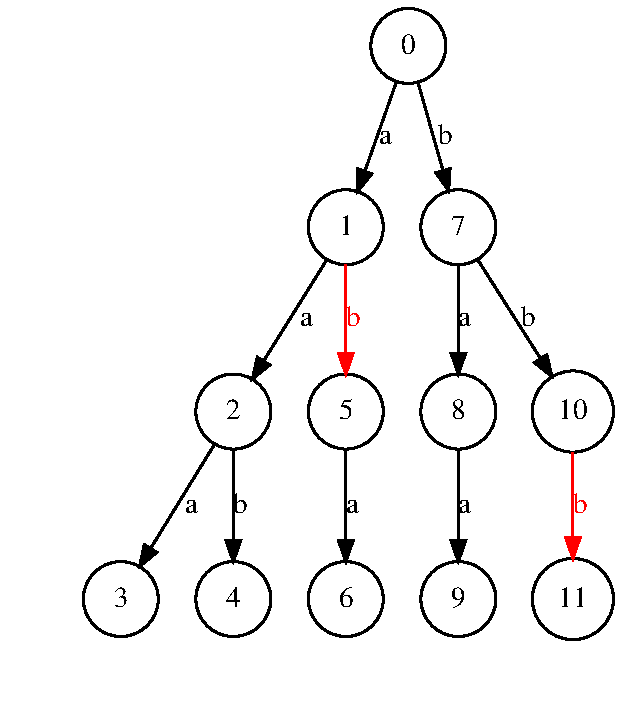
\includegraphics[height=0.6\textheight]{images/HTree07_c}}%
%\only<14>{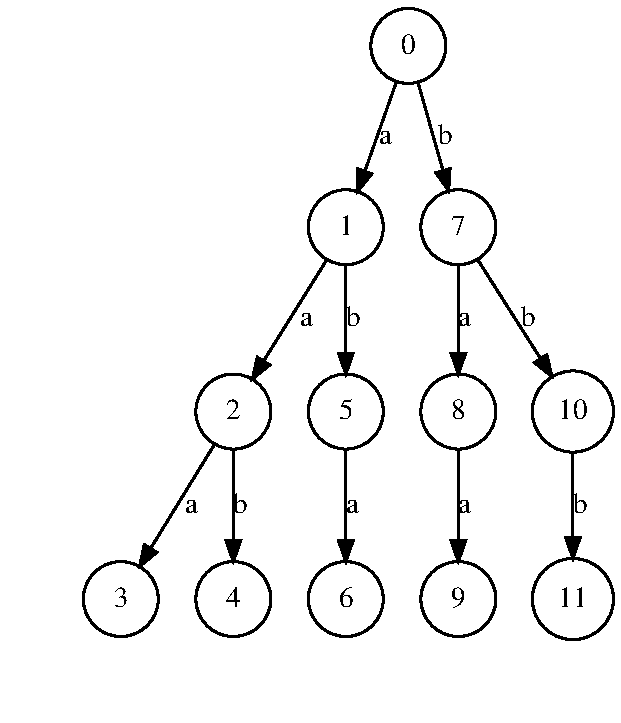
\includegraphics[height=0.6\textheight]{images/HTree07}}%
\end{column}%

\end{columns}
\end{frame}

\begin{frame}
\frametitle{$H$-Methode - Vergleich}
\begin{columns}[T] % align columns

\begin{column}{.50\textwidth}
\begin{itemize}
    \item $W$-Methode:\\8 Testfälle, 24 Testschritte
    \item $W_p$-Methode:\\7 Testfälle, 21 Testschritte
    \item $H$-Methode:\\  5 Testfälle, 15 Testschritte
\end{itemize}
\end{column}%

\begin{column}{.50\textwidth}
\centering
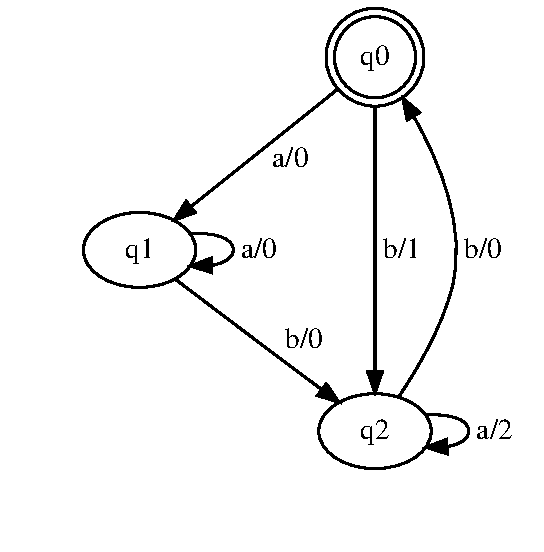
\includegraphics[width=\textwidth]{images/fsm-example01_orig}%
\end{column}%

\end{columns}
\end{frame}

%
%\begin{frame}
%\frametitle{$H$-Methode - Optimierung}
%Wahl von $\omega$ vom aktuellen Testbaum abhängig machen.

%\begin{itemize}
%      \item<2-> Ideal: Für $(\alpha, \beta$) finde $\omega$, sodass $\alpha.\omega$ und $\beta.\omega$ im Testbaum
%      \item<3-> Sonst: Erweitere bestehenden Test
%      \item<4-> Wenn nicht anders möglich: Neuer Testfall 
%    \end{itemize}
%\end{frame}

%\begin{frame}
%  \frametitle{$H$-Methode - Optimierung}

%  \begin{columns}[T] % align columns
%    \begin{column}{.3\textwidth}
%	    \begin{itemize}
%		  \item Betrachte $(c.a,d)$
%		  \item mögliches $\omega: e$
%	    \end{itemize}
%    \end{column}%

%    \begin{column}{.70\textwidth}
%        \only<1->{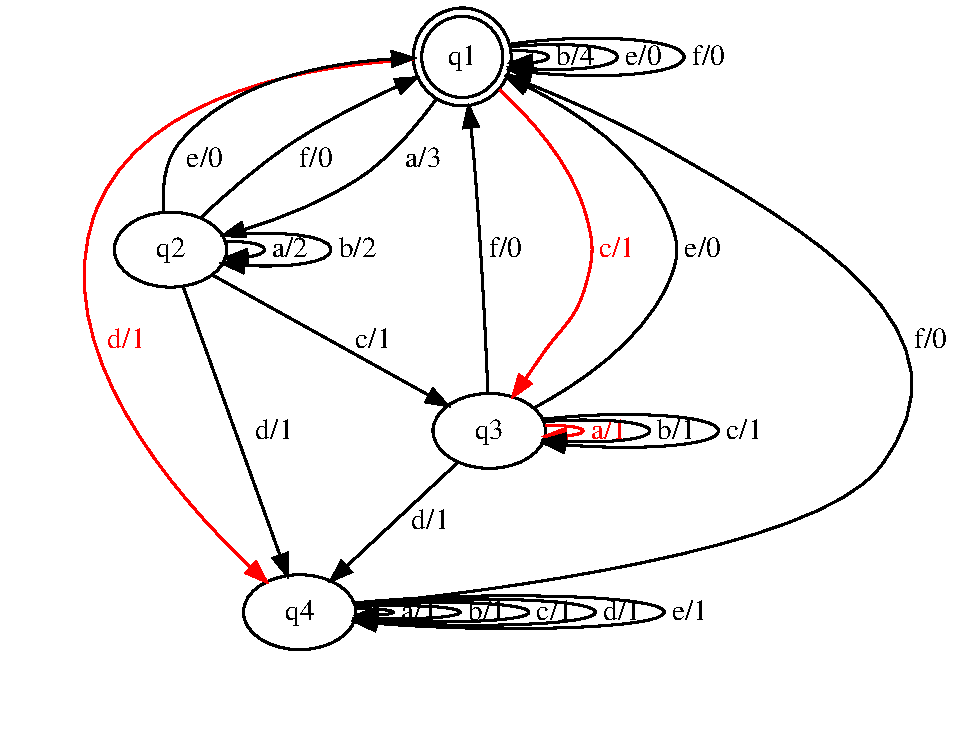
\includegraphics[width=\textwidth]{images/FSM_opt}}
%    \end{column}%
%  \end{columns}
%\end{frame}


%\begin{frame}
 % \frametitle{$H$-Methode - Optimierung}
 % \begin{columns}[T] % align columns

%\begin{column}{.4\textwidth}
%  \begin{itemize}
%	\item<2->Wahl $e$ für $\omega$ würde neuen Test erzeugen
%	\item<3->Versuche bestehenden Test zu erweitern
%	\item<4->$a.e$ statt $e$
%  \end{itemize}
%\end{column}%

%\begin{column}{.70\textwidth}
%Zu diesem Zeitpunkt sieht der Testbaum so aus:
%\only<1>{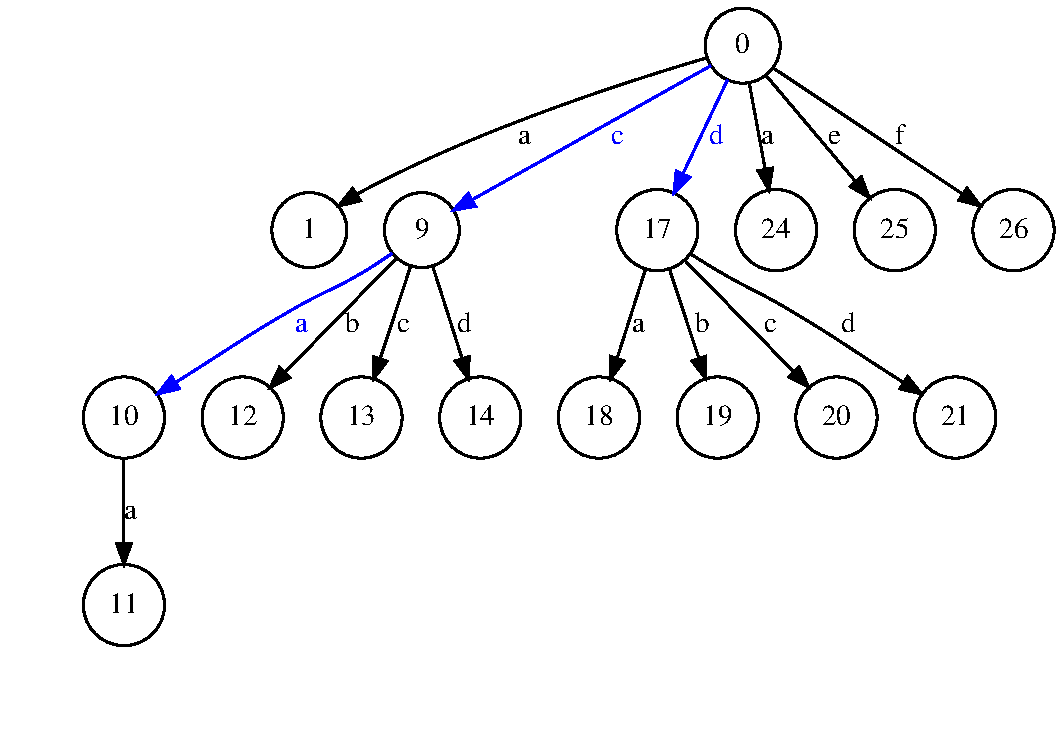
\includegraphics[height=0.6\textheight]{images/HTree_opt}}
%\only<2-3>{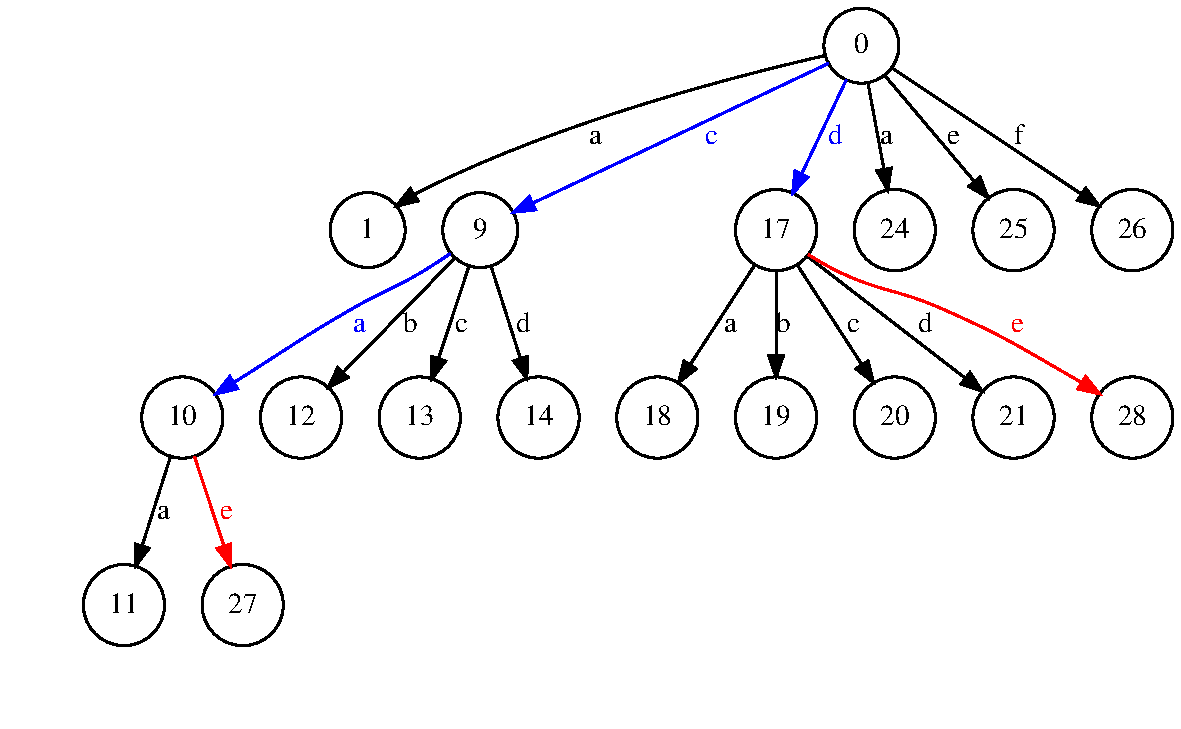
\includegraphics[height=0.6\textheight]{images/HTree_opt2}}
%\only<4->{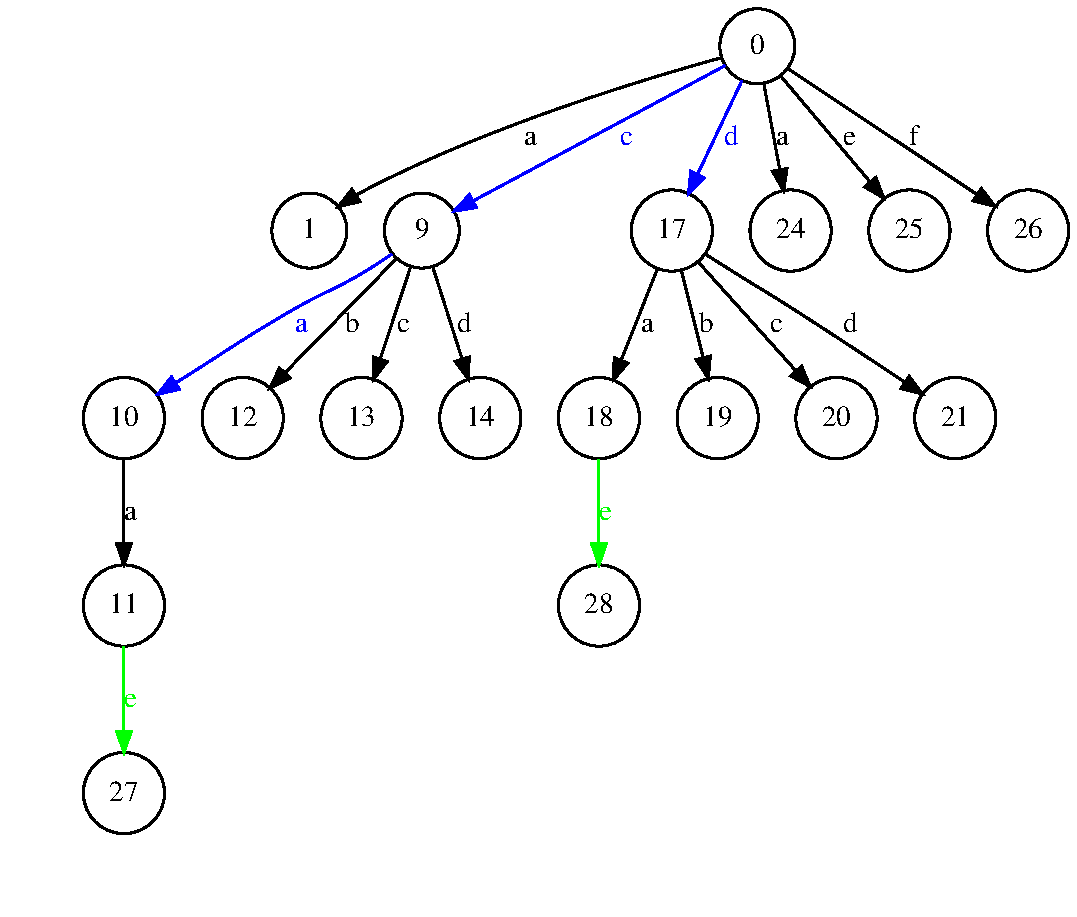
\includegraphics[height=0.7\textheight]{images/HTree_opt3}}
%\end{column}%

%\end{columns}

%\end{frame}
\section{Sicherheitsvollständige Testsuite}
\begin{frame}
\frametitle{Safety-related Output Abstraction}
\begin{itemize}
  \item<1-> Reaktion des Systems wird durch DFSM-Ausgabe modelliert
  \item<2-> Idee: Falsche Ausgabe muss nicht sicherheitsrelevant sein
  \item<3-> Sicherheitskritische Reaktionen definieren
  \item<4-> Nicht-sicherheitskritische Reaktionen zusammenfassen
\end{itemize}
\end{frame}

\begin{frame}
\frametitle{safety-Äquivalenz}
\begin{itemize}
  \item<1-> \emph{safety related output abstraction}: $\leq_s \subseteq \Sigma_O \times \Sigma_O$
  \item<2-> $\leq_s$ sei reflexiv, transitiv.
  \item<3-> s-äquivalent: $y_1 \sim_s y_2 \equiv y_1 \leq_s y_2$ und $y_2 \leq_s y_1$
  \item<4-> Zwei I/O-Folgen $X/Y, X'/Y'$ sind s-äquivalent gdw. $X=X'$ und $Y$ und $Y'$ sind s-äquivalent
  \item<5-> Zwei Zustände $q, q'$ sind s-äquivalent gdw. die Outputs für jede Inputfolge s-äquivalent sind.
  \item<6-> Zwei Systeme sind s-äquivalent gdw. ihre Anfangszustände s-äquivalent sind.
\end{itemize}
\end{frame}

\begin{frame}
\frametitle{Safety-Complete Test Suite}
Eine Test Suite $TS$ wird \emph{safety complete} genannt, gdw. für jede IUT $M'$ der Fehlerdomain gilt:
\begin{itemize}
  \item<1-> Soundness: $M$ und $M'$ sind I/O-äquivalent zueinander $\Rightarrow$ $M'$ besteht die Teset Suite ($M'~ \underline{pass}~ TS$)
  \item<2-> safety-Exhaustiveness: Für alle $M'$ aus der Fehlerdomain gilt: $M' \not \sim_s M \Rightarrow M'~ \underline{fail}~ TS$
\end{itemize}
\end{frame}

\begin{frame}
\frametitle{Beispiel}
\begin{columns}[T] % align columns

\begin{column}{.50\textwidth}
\textbf{M}
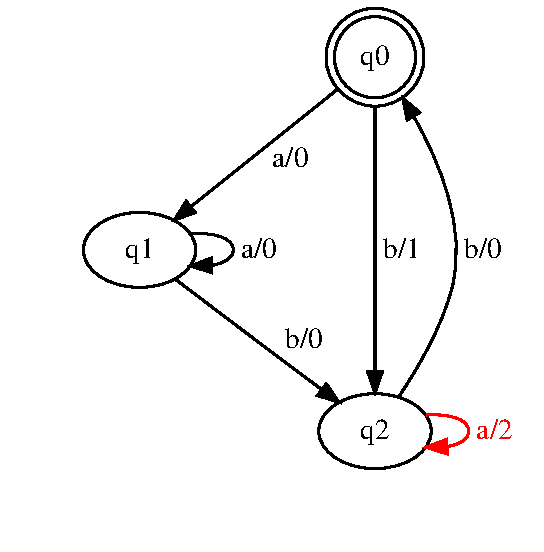
\includegraphics[width=\textwidth]{images/fsm-example01}
\end{column}%

\begin{column}{.50\textwidth}
\textbf{Safety Abstraktion von M}\\
\begin{itemize}
\item Ausgaben $0,1$  $\rightarrow Y$
\item Ausgabe $2$ ist safety-relevant: unverändert lassen
\end{itemize}
\end{column}%
\end{columns}
\end{frame}



\begin{frame}
\frametitle{Beispiel}
\begin{columns}[T] % align columns

\begin{column}{.50\textwidth}
\textbf{M}
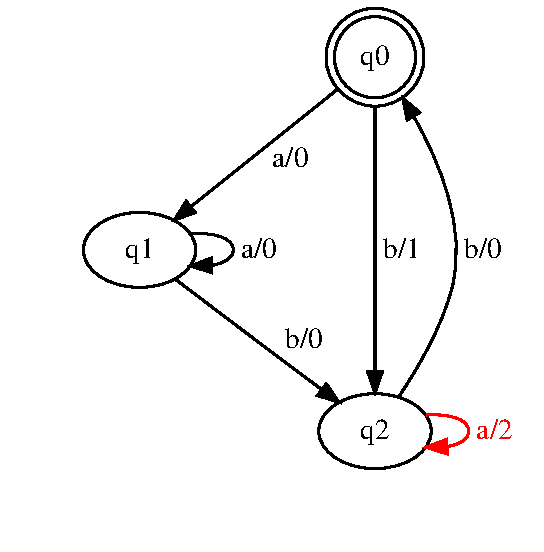
\includegraphics[width=\textwidth]{images/fsm-example01}
\end{column}%

\begin{column}{.50\textwidth}
\textbf{Safety Abstraktion von M}
\only<1>{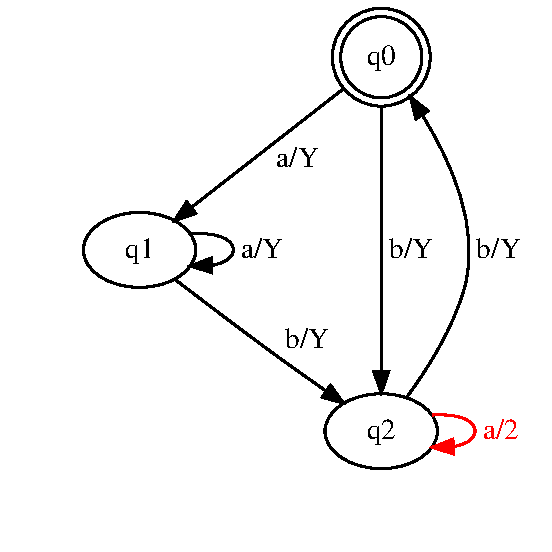
\includegraphics[width=\textwidth]{images/fsm-example01_abs}}%
\only<2->{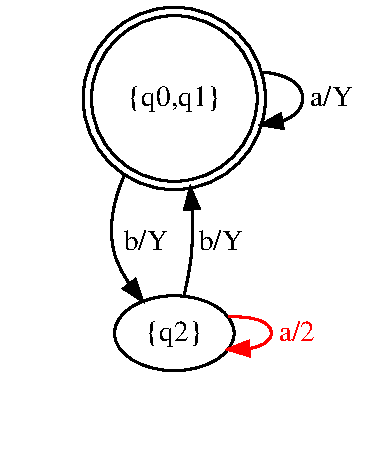
\includegraphics[width=0.8\textwidth]{images/fsm-example01_abs_min}}%
\end{column}%
\end{columns}
\end{frame}
\section{Algorithmen}

\begin{frame}
  \frametitle{Kosten beim Hinzufügen eines Tests}
  \begin{description}
    \item[$0$,] falls $\alpha.\gamma\in\pref(H_s)$ und $\beta.\gamma\in\pref(H_s)$. 
    \item[$1$,] falls $\alpha.\gamma\in\pref(H_s)$ und $\beta.\gamma$ erweitert eine bestehende Sequenz in $H_s$ oder umgekehrt.
    \item[$2$,] falls $\alpha.\gamma\not\in\pref(H_s)$ und $\beta.\gamma\not\in\pref(H_s)$, aber beide erweitern je eine bestehende Sequenz in $H_s$.
    \item[$3$,] falls $\alpha.\gamma\in\pref(H_s)$ und $\beta.\gamma$ ist nicht in $\pref(H_s)$ enthalten und erweitert auch keine bestehende Sequenz aus  $H_s$ oder umgekehrt.
    \item[$4$,] falls $\alpha.\gamma$ eine bestehende Sequenz in $H_s$ erweitert und $\beta.\gamma$ nicht in $\pref(H_s)$ enthalten ist und auch keine bestehende Sequenz aus $H_s$ erweitert, oder umgekehrt.
    \item[$5$,] falls sowohl  $\alpha.\gamma$ als auch $\beta.\gamma$ zu neuen Tests führen.
\end{description}
\end{frame}
    
\begin{frame}
  \frametitle{Algorithmus 1}
  \begin{itemize}
    \item Berechne die Mengen $A,B,C$.
    \item Berechne für jedes Paar von unterscheibaren Zuständen unterscheidenden Sequenzen aus den $P_k$-Tabellen:
    Betrachte die erste $P_k$-Tabelle, in denen sich die beiden Zielzustände in verschiedenen Äquivalenzklassen befinden, und berechne unterscheidende Sequenz 'rückwärts'.
    \item Überspringe Paare aus $B$ und $C$, wenn ihre Zielzustände sicherheitsäquivalent sind.
    \item Wähle ein $\gamma$ aus der vorberechneten Menge, sodass die Kosten beim Hinzufügen von $\alpha.\gamma$ und $\beta.\gamma$ minimal sind.
    \item Füge $\alpha.\gamma$ und $\beta.\gamma$ der Testsuite hinzu.
  \end{itemize}
\end{frame}

\begin{frame}
  \frametitle{Präfixrelationssequenzen}
  \begin{figure}
    \begin{subfigure}[c]{0.4\textwidth}
        \centering
        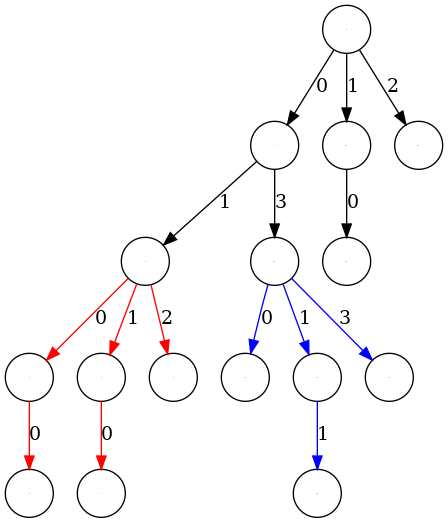
\includegraphics[width=\textwidth,height=5cm,keepaspectratio]{images/PRS_HS}
        \subcaption{Testsuite im Bearbeitungsschritt von $(\alpha,\beta)~=~(0.1,0.3)$.}
    \end{subfigure}
    \begin{subfigure}[c]{0.4\textwidth}
        \centering
        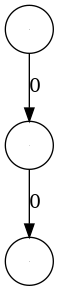
\includegraphics[width=\textwidth,height=5cm,keepaspectratio]{images/PRS_PRS}
        \subcaption{Präfixrelationssequenzen.}
    \end{subfigure}
\end{figure}
\end{frame}

\begin{frame}
  \frametitle{Algorithmus 2}
  \begin{itemize}
    \item Berechne die Mengen $A,B,C$.
    \item Initialisiere Testsuite: $H_s \gets V.\bigcup_{i=1}^{m-n+1}\Sigma_I^i$
    \item Überspringe Paare aus $B$ und $C$, wenn ihre Zielzustände sicherheitsäquivalent sind.
    \item Wähle $\gamma \in PRS(H_s,\alpha,\beta)$.
    \item Falls kein $\gamma$ gefunden werden kann, finde ein Element $x$ aus den PRS, sodass $\alpha.x$ und $\beta.x$ in unterschiedliche Zielzustände führen. Verlängere $x$ zu einer unterscheidenden Sequenz $\gamma$.
    \item Falls kein solches $x$ gefunden werden kann, berechne beliebige unterscheidende Sequenz $\gamma$.
    \item Füge $\alpha.\gamma$ und $\beta.\gamma$ der Testsuite hinzu.
  \end{itemize}
\end{frame}

\begin{frame}
  \frametitle{Algorithmus 3}
  Betrachte Präfixdurchschnittssequenzen
  \begin{itemize}
    \item Durchschnitt zweier Subbäume mit Präfix $\alpha$ bzw. $\beta$ kann immer hinzugefügt werden, ist aber nicht in den PRS enthalten.
    \item Dadurch werden günstige unterscheidende Sequenzen vernachlässigt
    $$PDS = PRS \cup \big( \pref(\successor(\alpha)_{H_s}) \cap \pref(\successor(\beta)_{H_s}) \big) $$
    \item Erhöhter Aufwand
    \item Einziger Unterschied zu Algorithmus 2: Wähle $\gamma \in PDS(H_s,\alpha,\beta)$.
  \end{itemize}
\end{frame}
\section{Evaluation}

\begin{frame}
  \frametitle{Fasten-Seat-Belt}
  \begin{table}[]
    \caption{Ergebnisse für die \glqq Fasten-Seat-Belt\grqq-DFSM.}
    \label{tab:fsbrtsx}
    \centering
    \begin{tabular}{|ccccc|}
    \hline
          & \#Testfälle & \#Testschritte & ms & $\text{RED}_H$\\ \hline\hline
        $\text{s-H}_1$ & 337         & 1487    &    23   &  31\% \\ \hline
    $\text{s-H}_2$ & 423         & 2835    &    285  & 34\%  \\ \hline
    $\text{s-H}_3$ & 399         & 2558    &    372   &  36\% \\ \hline
    \end{tabular}
\end{table}
\end{frame} 

\begin{frame}
  \frametitle{Statistische Experimente}
  \begin{itemize}
    \item Konstruktion von Referenzmodell und Abstraktionsmodell.
  \end{itemize}
  \begin{table}[]
    \centering
    \begin{tabular}{|l|l|l|l|l|}
    \hline
    \textbf{$|Abs_{min}|$} & \textbf{$|Ref_{min}|$} & \textbf{$\Sigma_I$}   & \textbf{$\Sigma_O$}  & \textbf{$m-n$}   \\ \hline
    [2--99]     & 100        & 4      & 8      & 0 \\ \hline
    4          & [10--100]   & 4      & 8      & 0 \\ \hline
    4          & 20         & [2--10] & 8      & 0 \\ \hline
    4          & 20         & 4      & [3--20] & 0 \\ \hline
    4          & 20         & 4      & 8      & [0--3] \\ \hline
    \end{tabular}
    \caption{Versuchsaufbau für die statistischen Experimente. 100 Durchläufe pro Experiment.}
\end{table}
\end{frame}


\begin{frame}
  \frametitle{Konstruktion 1 (modulo)}
  \begin{itemize}
    \item Konstruiere Referenzmodell $M$ mit $n$ Zuständen, Abstraktionsmodell $M'$ mit $m$ Zuständen.
    \item Nummeriere Zustände.
    \item Teile die Zustände des Referenzmodells in $m$ Äquivalenzklassen ein ($q_n \mod m$).
    \item Wähle $0$ als sicherheitskritische Ausgabe, alle anderen Ausgaben sicherheitsäquivalent zueinander.
    \item Belege leere Transitionstabelle mit zufälligen Werten.
    \item Füge nach jeder Belegung notwendige Implikationen durch.
  \end{itemize}
\end{frame}


\begin{frame}
  \frametitle{Konstruktion 1 (modulo)}
  \centering
  \begin{tabular}{cc}
    \begin{tabular}{|l|l|l|l|l|}
      \hline
      & \multicolumn{2}{l|}{I2O} & \multicolumn{2}{l|}{I2P} \\\hline
    q & a           & b          & a           & b          \\\hline\hline
    \cellcolor[HTML]{DAE8FC}0  &             &            &             &            \\\hline
    1 &             &            &             &            \\\hline
    \cellcolor[HTML]{DAE8FC}2 &             &            &             &            \\\hline
    3 &             &            &             &            \\\hline
    \cellcolor[HTML]{DAE8FC}4 &             &            &             &            \\\hline
    5 &             &            &             &            \\\hline
    \cellcolor[HTML]{DAE8FC}6 &             &            &             &            \\\hline
    7 &             &            &             &            \\\hline
    \cellcolor[HTML]{DAE8FC}8 &             &            &             &            \\\hline
    9 &             &            &             &           \\\hline
    \end{tabular}
    &
    \begin{tabular}{|r|r|r|r|r|}
      \hline
      & \multicolumn{2}{l|}{I2O} & \multicolumn{2}{l|}{I2P} \\\hline
    q & a           & b          & a           & b          \\\hline\hline
    \cellcolor[HTML]{DAE8FC}$0:=\{0,2,4,6,8\}$  &             &            &             &            \\\hline
    $1:=\{1,3,5,7,9\}$ &             &            &             &            \\\hline
    \end{tabular}
    \end{tabular}
\end{frame}

\begin{frame}
  \frametitle{Konstruktion 1 (modulo)}
  \centering
  \begin{tabular}{cc}
    \begin{tabular}{|l|l|l|l|l|}
      \hline
      & \multicolumn{2}{l|}{I2O} & \multicolumn{2}{l|}{I2P} \\\hline
    q & a           & b          & a           & b          \\\hline\hline
    \cellcolor[HTML]{DAE8FC}0  &  1           &            & 4            &            \\\hline
    1 &             &            &             &            \\\hline
    \cellcolor[HTML]{DAE8FC}2 &             &            &             &            \\\hline
    3 &             &            &             &            \\\hline
    \cellcolor[HTML]{DAE8FC}4 &             &            &             &            \\\hline
    5 &             &            &             &            \\\hline
    \cellcolor[HTML]{DAE8FC}6 &             &            &             &            \\\hline
    7 &             &            &             &            \\\hline
    \cellcolor[HTML]{DAE8FC}8 &             &            &             &            \\\hline
    9 &             &            &             &           \\\hline
    \end{tabular}
    &
    \begin{tabular}{|r|r|r|r|r|}
      \hline
      & \multicolumn{2}{l|}{I2O} & \multicolumn{2}{l|}{I2P} \\\hline
    q & a           & b          & a           & b          \\\hline\hline
    \cellcolor[HTML]{DAE8FC}$0:=\{0,2,4,6,8\}$  &             &            &             &            \\\hline
    $1:=\{1,3,5,7,9\}$ &             &            &             &            \\\hline
    \end{tabular}
    \end{tabular}
\end{frame}

\begin{frame}
  \frametitle{Konstruktion 1 (modulo)}
  \centering
  \begin{tabular}{cc}
    \begin{tabular}{|l|l|l|l|l|}
      \hline
      & \multicolumn{2}{l|}{I2O} & \multicolumn{2}{l|}{I2P} \\\hline
    q & a           & b          & a           & b          \\\hline\hline
    \cellcolor[HTML]{DAE8FC}0  & 1            &            &  4           &            \\\hline
    1 &             &            &             &            \\\hline
    \cellcolor[HTML]{DAE8FC}2 &  3           &            & 2            &            \\\hline
    3 &             &            &             &            \\\hline
    \cellcolor[HTML]{DAE8FC}4 &  1           &            & 2            &            \\\hline
    5 &             &            &             &            \\\hline
    \cellcolor[HTML]{DAE8FC}6 &  2           &            & 8            &            \\\hline
    7 &             &            &             &            \\\hline
    \cellcolor[HTML]{DAE8FC}8 &  2           &            & 0            &            \\\hline
    9 &             &            &             &           \\\hline
    \end{tabular}
    &
    \begin{tabular}{|r|r|r|r|r|}
      \hline
      & \multicolumn{2}{l|}{I2O} & \multicolumn{2}{l|}{I2P} \\\hline
    q & a           & b          & a           & b          \\\hline\hline
    \cellcolor[HTML]{DAE8FC}$0:=\{0,2,4,6,8\}$  & Y            &           & $0$            &            \\\hline
    $1:=\{1,3,5,7,9\}$ &             &            &             &            \\\hline
    \end{tabular}
    \end{tabular}
\end{frame}

\begin{frame}
  \frametitle{Konstruktion 1 (modulo)}
  \centering
  \begin{tabular}{cc}
    \begin{tabular}{|l|l|l|l|l|}
      \hline
      & \multicolumn{2}{l|}{I2O} & \multicolumn{2}{l|}{I2P} \\\hline
    q & a           & b          & a           & b          \\\hline\hline
    \cellcolor[HTML]{DAE8FC}0  & 1            &  0          &  4           &  3          \\\hline
    1 &             &            &             &            \\\hline
    \cellcolor[HTML]{DAE8FC}2 &  3           &            & 2            &            \\\hline
    3 &             &            &             &            \\\hline
    \cellcolor[HTML]{DAE8FC}4 &  1           &            & 2            &            \\\hline
    5 &             &            &             &            \\\hline
    \cellcolor[HTML]{DAE8FC}6 &  2           &            & 8            &            \\\hline
    7 &             &            &             &            \\\hline
    \cellcolor[HTML]{DAE8FC}8 &  2           &            & 0            &            \\\hline
    9 &             &            &             &           \\\hline
    \end{tabular}
    &
    \begin{tabular}{|r|r|r|r|r|}
      \hline
      & \multicolumn{2}{l|}{I2O} & \multicolumn{2}{l|}{I2P} \\\hline
    q & a           & b          & a           & b          \\\hline\hline
    \cellcolor[HTML]{DAE8FC}$0:=\{0,2,4,6,8\}$  & Y            &           & $0$            &            \\\hline
    $1:=\{1,3,5,7,9\}$ &             &            &             &            \\\hline
    \end{tabular}
    \end{tabular}
\end{frame}


\begin{frame}
  \frametitle{Konstruktion 1 (modulo)}
  \centering
  \begin{tabular}{cc}
    \begin{tabular}{|l|l|l|l|l|}
      \hline
      & \multicolumn{2}{l|}{I2O} & \multicolumn{2}{l|}{I2P} \\\hline
    q & a           & b          & a           & b          \\\hline\hline
    \cellcolor[HTML]{DAE8FC}0  & 1            &  0          &  4           &  3          \\\hline
    1 &             &            &             &            \\\hline
    \cellcolor[HTML]{DAE8FC}2 &  3           & 0           & 2            &  1          \\\hline
    3 &             &            &             &            \\\hline
    \cellcolor[HTML]{DAE8FC}4 &  1           & 0           & 2            &  7          \\\hline
    5 &             &            &             &            \\\hline
    \cellcolor[HTML]{DAE8FC}6 &  2           & 0           & 8            &  3          \\\hline
    7 &             &            &             &            \\\hline
    \cellcolor[HTML]{DAE8FC}8 &  2           & 0           & 0            &  3          \\\hline
    9 &             &            &             &           \\\hline
    \end{tabular}
    &
    \begin{tabular}{|r|r|r|r|r|}
      \hline
      
      & \multicolumn{2}{l|}{I2O} & \multicolumn{2}{l|}{I2P} \\\hline
    q & a           & b          & a           & b          \\\hline\hline
    \cellcolor[HTML]{DAE8FC}$0:=\{0,2,4,6,8\}$  & Y            & 0          & $0$ & $1$           \\\hline
    $1:=\{1,3,5,7,9\}$ &             &            &             &            \\\hline
    \end{tabular}
    \end{tabular}
\end{frame}


\begin{frame}
  \frametitle{Konstruktion 2 (extreme)}
  \centering
  \begin{tabular}{cc}
    \begin{tabular}{|l|l|l|l|l|}
      \hline
      & \multicolumn{2}{l|}{I2O} & \multicolumn{2}{l|}{I2P} \\\hline
    q & a           & b          & a           & b          \\\hline\hline
    0  &             &            &             &            \\\hline
    \cellcolor[HTML]{DAE8FC}1 &             &            &             &            \\\hline
    \cellcolor[HTML]{DAE8FC}2 &             &            &             &            \\\hline
    \cellcolor[HTML]{DAE8FC}3 &             &            &             &            \\\hline
    \cellcolor[HTML]{DAE8FC}4 &             &            &             &            \\\hline
    \cellcolor[HTML]{DAE8FC}5 &             &            &             &            \\\hline
    \cellcolor[HTML]{DAE8FC}6 &             &            &             &            \\\hline
    \cellcolor[HTML]{DAE8FC}7 &             &            &             &            \\\hline
    \cellcolor[HTML]{DAE8FC}8 &             &            &             &            \\\hline
    \cellcolor[HTML]{DAE8FC}9 &             &            &             &           \\\hline
    \end{tabular}
    &
    \begin{tabular}{|r|r|r|r|r|}
      \hline
      & \multicolumn{2}{l|}{I2O} & \multicolumn{2}{l|}{I2P} \\\hline
    q & a           & b          & a           & b          \\\hline\hline
    \cellcolor[HTML]{DAE8FC}$0$  &             &            &             &            \\\hline
    $1:=\{1,2,3,4,5,6,7,8,9\}$ &             &            &             &            \\\hline
    \end{tabular}
    \end{tabular}
\end{frame}

\begin{frame}
  \frametitle{$|Abs_{min}|$ -- Anzahl der Tests}
  \footnotesize Ref$_{min} = 100$, $\Sigma_I=4, \Sigma_O=8, m=n$
  \normalsize
\pgfplotsset{width=3.5cm,height=3.5cm}
\begin{center}
    \begin{minipage}{\linewidth}
        \centering

        \begin{tikzpicture}
        \pgfplotsset{compat=newest}
        \definecolor{clr1}{RGB}{250,100,25}
        \definecolor{clr2}{RGB}{100,25,250}
        \definecolor{clr3}{RGB}{25,250,100}
        \definecolor{clr4}{RGB}{150,85,20}
        \definecolor{clr5}{RGB}{85,20,150}
        \definecolor{clr6}{RGB}{20,150,85}
        %\begin{axis}[ legend style={at={(1,1)},xshift=0.5cm,anchor=north west},scale only axis, xmin=3, xmax=20, xlabel={$|\Sigma_I|$}, ylabel={$\#$Test Cases}]%
        \begin{axis}[ legend pos = north west,scale only axis, xmin=2, xmax=45, xlabel={$|Abs_{min}|$}, ylabel={$\#$Tests}]%
            \addplot[mark=square*,mark options={scale=0.3},clr1] table [x=absMin,y=Size_SH1] {data/c1_modulo};
            \label{plot_sh1} \addlegendentry{$\text{s-H}_1$}
            \addplot[mark=square*,mark options={scale=0.3},clr2] table [x=absMin,y=Size_SH2] {data/c1_modulo};
            \label{plot_sh2} \addlegendentry{$\text{s-H}_2$}
            \addplot[mark=square*,mark options={scale=0.3},clr3] table [x=absMin,y=Size_SH3] {data/c1_modulo};
            \label{plot_sh3} \addlegendentry{$\text{s-H}_3$}
        \end{axis}
        \end{tikzpicture}
        \begin{tikzpicture}
            \pgfplotsset{compat=newest}
            \definecolor{clr1}{RGB}{250,100,25}
            \definecolor{clr2}{RGB}{100,25,250}
            \definecolor{clr3}{RGB}{25,250,100}
            \definecolor{clr4}{RGB}{225,85,20}
            \definecolor{clr5}{RGB}{85,20,225}
            \definecolor{clr6}{RGB}{20,225,85}
            %\begin{axis}[ legend style={at={(1,1)},xshift=0.5cm,anchor=north west},scale only axis, xmin=3, xmax=20, xlabel={$|\Sigma_I|$}, ylabel={$\#$Test Cases}]%
            \begin{axis}[scale only axis, xmin=2, xmax=99, xlabel={$|Abs_{min}|$}]%
                \addplot[mark=square*,mark options={scale=0.2},clr1] table [x=absMin,y=Size_SH1] {data/c1_extreme};
                \addplot[mark=square*,mark options={scale=0.2},clr2] table [x=absMin,y=Size_SH2] {data/c1_extreme};
                \addplot[mark=square*,mark options={scale=0.2},clr3] table [x=absMin,y=Size_SH3] {data/c1_extreme};
            \end{axis}
        \end{tikzpicture}
        %}
        \captionof{figure}{Anzahl der Tests in Abhängigkeit von $|Abs_{min}|$, links: modulo-Konstruktion, rechts: extreme-Konstruktion}
    \end{minipage}
    \end{center}
%%%%%%%%%%
\end{frame}

\begin{frame}
  
\pgfplotsset{width=3.5cm,height=3.5cm}
\begin{center}
  \frametitle{$|Abs_{min}|$ -- Anzahl der Testschritte}
  \footnotesize Ref$_{min} = 100$, $\Sigma_I=4, \Sigma_O=8, m=n$
  \normalsize
    \begin{minipage}{\linewidth}
        \centering
        \begin{tikzpicture}
        \pgfplotsset{compat=newest}
        \definecolor{clr1}{RGB}{250,100,25}
        \definecolor{clr2}{RGB}{100,25,250}
        \definecolor{clr3}{RGB}{25,250,100}
        \definecolor{clr4}{RGB}{225,85,20}
        \definecolor{clr5}{RGB}{85,20,225}
        \definecolor{clr6}{RGB}{20,225,85}
        %\begin{axis}[ legend style={at={(1,1)},xshift=0.5cm,anchor=north west},scale only axis, xmin=3, xmax=20, xlabel={$|\Sigma_I|$}, ylabel={$\#$Test Cases}]%
        \begin{axis}[ scale only axis, xmin=2, xmax=99, xlabel={$|Abs_{min}|$}, ylabel={$\#$Testschritte}]%
            \addplot[mark=square*,mark options={scale=0.3},clr1] table [x=absMin,y=Total_SH1] {data/c1_modulo};
            \addplot[mark=square*,mark options={scale=0.3},clr2] table [x=absMin,y=Total_SH2] {data/c1_modulo};
            \addplot[mark=square*,mark options={scale=0.3},clr3] table [x=absMin,y=Total_SH3] {data/c1_modulo};
        \end{axis}
        \end{tikzpicture}
        \begin{tikzpicture}
        \pgfplotsset{compat=newest}
        \definecolor{clr1}{RGB}{250,100,25}
        \definecolor{clr2}{RGB}{100,25,250}
        \definecolor{clr3}{RGB}{25,250,100}
        \definecolor{clr4}{RGB}{225,85,20}
        \definecolor{clr5}{RGB}{85,20,225}
        \definecolor{clr6}{RGB}{20,225,85}
        %\begin{axis}[ legend style={at={(1,1)},xshift=0.5cm,anchor=north west},scale only axis, xmin=3, xmax=20, xlabel={$|\Sigma_I|$}, ylabel={$\#$Test Cases}]%
        \begin{axis}[ legend pos = south east, scale only axis, xmin=2, xmax=99, xlabel={$|Abs_{min}|$}]%
            \addplot[mark=square*,mark options={scale=0.3},clr1] table [x=absMin,y=Total_SH1] {data/c1_extreme};
            \label{plot_sh1} \addlegendentry{$\text{s-H}_1$}
            \addplot[mark=square*,mark options={scale=0.3},clr2] table [x=absMin,y=Total_SH2] {data/c1_extreme};
            \label{plot_sh2} \addlegendentry{$\text{s-H}_2$}
            \addplot[mark=square*,mark options={scale=0.3},clr3] table [x=absMin,y=Total_SH3] {data/c1_extreme};
            \label{plot_sh3} \addlegendentry{$\text{s-H}_3$}
        \end{axis}
        \end{tikzpicture}
        %}
        \captionof{figure}{\label{fig:c1_red_total}Anzahl der Testschritte in Abhängigkeit von $|Abs_{min}|$,
        links: modulo-Konstruktion, rechts: extreme-Konstruktion}
    \end{minipage}
    \end{center}
\end{frame}

\begin{frame}
  \frametitle{$|Abs_{min}|$ -- Testreduktion}
  \footnotesize Ref$_{min} = 100$, $\Sigma_I=4, \Sigma_O=8, m=n$
  \normalsize
  \pgfplotsset{width=3.5cm,height=3.5cm}
  \begin{center}
      \begin{minipage}{\linewidth}
          \centering
          \begin{tikzpicture}
          \pgfplotsset{compat=newest}
          \definecolor{clr1}{RGB}{250,100,25}
          \definecolor{clr2}{RGB}{100,25,250}
          \definecolor{clr3}{RGB}{25,250,100}
          \definecolor{clr4}{RGB}{225,85,20}
          \definecolor{clr5}{RGB}{85,20,225}
          \definecolor{clr6}{RGB}{20,225,85}
          %\begin{axis}[ legend style={at={(1,1)},xshift=0.5cm,anchor=north west},scale only axis, xmin=3, xmax=20, xlabel={$|\Sigma_I|$}, ylabel={$\#$Test Cases}]%
          \begin{axis}[ scale only axis, xmin=2, xmax=35, xlabel={$|Abs_{min}|$}, ylabel={$\mathbf{Red_H\%}$}]%
              \addplot[mark=square*,mark options={scale=0.2},clr1] table [x=absMin,y=Impr_SH1] {data/c1_modulo};
              \addplot[mark=square*,mark options={scale=0.2},clr2] table [x=absMin,y=Impr_SH2] {data/c1_modulo};
              \addplot[mark=square*,mark options={scale=0.2},clr3] table [x=absMin,y=Impr_SH3] {data/c1_modulo};
              
          \end{axis}
          \end{tikzpicture}
          \begin{tikzpicture}
          \pgfplotsset{compat=newest}
          \definecolor{clr1}{RGB}{250,100,25}
          \definecolor{clr2}{RGB}{100,25,250}
          \definecolor{clr3}{RGB}{25,250,100}
          \definecolor{clr4}{RGB}{225,85,20}
          \definecolor{clr5}{RGB}{85,20,225}
          \definecolor{clr6}{RGB}{20,225,85}
          %\begin{axis}[ legend style={at={(1,1)},xshift=0.5cm,anchor=north west},scale only axis, xmin=3, xmax=20, xlabel={$|\Sigma_I|$}, ylabel={$\#$Test Cases}]%
          \begin{axis}[ legend pos = north east, scale only axis, xmin=2, xmax=50, xlabel={$|Abs_{min}|$}]%
              \addplot[mark=square*,mark options={scale=0.2},clr1] table [x=absMin,y=Impr_SH1] {data/c1_extreme};
              \label{plot_sh1} \addlegendentry{$\text{s-H}_1$}
              \addplot[mark=square*,mark options={scale=0.2},clr2] table [x=absMin,y=Impr_SH2] {data/c1_extreme};
              \label{plot_sh2} \addlegendentry{$\text{s-H}_2$}
              \addplot[mark=square*,mark options={scale=0.2},clr3] table [x=absMin,y=Impr_SH3] {data/c1_extreme};
              \label{plot_sh3} \addlegendentry{$\text{s-H}_3$}
          \end{axis}
          \end{tikzpicture}
          %}
          \captionof{figure}{\label{fig:c1_red_percent}Reduktion der Anzahl der Tests in Abhängigkeit von der Anzahl der Zustände des Abstraktionsmodells,
          links: modulo-Konstruktion, rechts: extreme-Konstruktion,
          $m=n$.}
      \end{minipage}
      \end{center}  
\end{frame}

\begin{frame}
  \frametitle{$|Abs_{min}|$ -- Laufzeit}
  \footnotesize Ref$_{min} = 100$, $\Sigma_I=4, \Sigma_O=8, m=n$
  \normalsize
\pgfplotsset{width=3.4cm,height=3.4cm,
yticklabel style={
    /pgf/number format/fixed,
    /pgf/number format/precision=5
},
scaled y ticks=false}

\begin{center}
\begin{minipage}{\linewidth}
    \centering
    \begin{tikzpicture}[baseline=(current axis.south)]
    \pgfplotsset{compat=newest}
    \definecolor{clr1}{RGB}{250,100,25}
    \definecolor{clr2}{RGB}{100,25,250}
    \definecolor{clr3}{RGB}{25,250,100}
    \definecolor{clr4}{RGB}{225,85,20}
    \definecolor{clr5}{RGB}{85,20,225}
    \definecolor{clr6}{RGB}{20,225,85}
    %\begin{axis}[ legend style={at={(1,1)},xshift=0.5cm,anchor=north west},scale only axis, xmin=3, xmax=20, xlabel={$|\Sigma_I|$}, ylabel={$\#$Test Cases}]%
    \begin{axis}[ scale only axis, xmin=2, xmax=99, xlabel={$|Abs_{min}|$}, ylabel={Zeit in ms}]%
      \addplot[mark=square*,mark options={scale=0.1},clr1] table [x=absMin,y=timeSH1] {data/c1_modulo};
      \label{plot_sh1} \addlegendentry{$\text{s-H}_1$}
      \addplot[mark=square*,mark options={scale=0.1},clr2] table [x=absMin,y=timeSH2] {data/c1_modulo};
      \label{plot_sh2} \addlegendentry{$\text{s-H}_2$}
      \addplot[mark=square*,mark options={scale=0.1},clr3] table [x=absMin,y=timeSH3] {data/c1_modulo};
      \label{plot_sh3} \addlegendentry{$\text{s-H}_3$}
    \end{axis}
    \end{tikzpicture}
    \begin{tikzpicture}[baseline=(current axis.south)]
        \pgfplotsset{compat=newest}
        \definecolor{clr1}{RGB}{250,100,25}
        \definecolor{clr2}{RGB}{100,25,250}
        \definecolor{clr3}{RGB}{25,250,100}
        \definecolor{clr4}{RGB}{225,85,20}
        \definecolor{clr5}{RGB}{85,20,225}
        \definecolor{clr6}{RGB}{20,225,85}
        %\begin{axis}[ legend style={at={(1,1)},xshift=0.5cm,anchor=north west},scale only axis, xmin=3, xmax=20, xlabel={$|\Sigma_I|$}, ylabel={$\#$Test Cases}]%
        \begin{axis}[legend pos = north west, scale only axis, xmin=2, xmax=99, xlabel={$|Abs_{min}|$}]%
          \addplot[mark=square*,mark options={scale=0.1},clr1] table [x=absMin,y=timeSH1] {data/c1_extreme};
          \addplot[mark=square*,mark options={scale=0.1},clr2] table [x=absMin,y=timeSH2] {data/c1_extreme};
          \addplot[mark=square*,mark options={scale=0.1},clr3] table [x=absMin,y=timeSH3] {data/c1_extreme};
        \end{axis}
        \end{tikzpicture}
    %}
    \captionof{figure}{\label{fig:c1_speed}Durchschnittliche Zeit in Millisekunden, die für die Testgenerierung in Abhängigkeit von $|Abs_{min}|$ benötigt wurde,
    links: modulo-Konstruktion, rechts: extreme-Konstruktion}
\end{minipage}
\end{center}
\end{frame}

\begin{frame}
  \frametitle{$|Ref_{min}|$ -- Anzahl der Tests}
  \footnotesize $|Abs_{min}| = 4$, $\Sigma_I=4, \Sigma_O=8, m=n$
  \normalsize
\pgfplotsset{width=3.5cm,height=3.5cm}
\begin{center}
    \begin{minipage}{\linewidth}
        \centering
        \begin{tikzpicture}
        \pgfplotsset{compat=newest}
        \definecolor{clr1}{RGB}{250,100,25}
        \definecolor{clr2}{RGB}{100,25,250}
        \definecolor{clr3}{RGB}{25,250,100}
        \definecolor{clr4}{RGB}{150,85,20}
        \definecolor{clr5}{RGB}{85,20,150}
        \definecolor{clr6}{RGB}{20,150,85}
        %\begin{axis}[ legend style={at={(1,1)},xshift=0.5cm,anchor=north west},scale only axis, xmin=3, xmax=20, xlabel={$|\Sigma_I|$}, ylabel={$\#$Test Cases}]%
        \begin{axis}[ legend pos = north west,scale only axis, xmin=10, xmax=100, xlabel={$|Ref_{min}|$}, ylabel={$\#$Tests}]%
            \addplot[mark=square*,mark options={scale=0.2},clr1] table [x=refMin,y=Size_SH1] {data/c2_modulo};
            \label{plot_sh1} \addlegendentry{$\text{s-H}_1$}
            \addplot[mark=square*,mark options={scale=0.2},clr2] table [x=refMin,y=Size_SH2] {data/c2_modulo};
            \label{plot_sh2} \addlegendentry{$\text{s-H}_2$}
            \addplot[mark=square*,mark options={scale=0.2},clr3] table [x=refMin,y=Size_SH3] {data/c2_modulo};
            \label{plot_sh3} \addlegendentry{$\text{s-H}_3$}
        \end{axis}
        \end{tikzpicture}
        \begin{tikzpicture}
            \pgfplotsset{compat=newest}
            \definecolor{clr1}{RGB}{250,100,25}
            \definecolor{clr2}{RGB}{100,25,250}
            \definecolor{clr3}{RGB}{25,250,100}
            \definecolor{clr4}{RGB}{225,85,20}
            \definecolor{clr5}{RGB}{85,20,225}
            \definecolor{clr6}{RGB}{20,225,85}
            %\begin{axis}[ legend style={at={(1,1)},xshift=0.5cm,anchor=north west},scale only axis, xmin=3, xmax=20, xlabel={$|\Sigma_I|$}, ylabel={$\#$Test Cases}]%
            \begin{axis}[scale only axis, xmin=10, xmax=100, xlabel={$|Ref_{min}|$}]%
                \addplot[mark=square*,mark options={scale=0.2},clr1] table [x=refMin,y=Size_SH1] {data/c2_extreme};
                \addplot[mark=square*,mark options={scale=0.2},clr2] table [x=refMin,y=Size_SH2] {data/c2_extreme};
                \addplot[mark=square*,mark options={scale=0.2},clr3] table [x=refMin,y=Size_SH3] {data/c2_extreme};
            \end{axis}
        \end{tikzpicture}
        %}
        \captionof{figure}{Anzahl der Tests in Abhängigkeit von der Anzahl der Zustände des Referenzmodells,
        links: modulo-Konstruktion, rechts: extreme-Konstruktion}
    \end{minipage}
    \end{center}
\end{frame}

\begin{frame}
  \frametitle{$|Ref_{min}|$ -- Testreduktion}
  \footnotesize $|Abs_{min}| = 4$, $\Sigma_I=4, \Sigma_O=8, m=n$
  \normalsize
\pgfplotsset{width=3.5cm,height=3.5cm}
\begin{center}
    \begin{minipage}{\linewidth}
        \centering
        \begin{tikzpicture}
        \pgfplotsset{compat=newest}
        \definecolor{clr1}{RGB}{250,100,25}
        \definecolor{clr2}{RGB}{100,25,250}
        \definecolor{clr3}{RGB}{25,250,100}
        \definecolor{clr4}{RGB}{225,85,20}
        \definecolor{clr5}{RGB}{85,20,225}
        \definecolor{clr6}{RGB}{20,225,85}
        %\begin{axis}[ legend style={at={(1,1)},xshift=0.5cm,anchor=north west},scale only axis, xmin=3, xmax=20, xlabel={$|\Sigma_I|$}, ylabel={$\#$Test Cases}]%
        \begin{axis}[  scale only axis, ymin=0,ymax=22,xmin=10, xmax=100, xlabel={$|Ref_{min}|$}, ylabel={$\mathbf{Red_H\%}$}]%
            \addplot[mark=square*,mark options={scale=0.3},clr1] table [x=refMin,y=Impr_SH1] {data/c2_modulo};
            
            \addplot[mark=square*,mark options={scale=0.3},clr2] table [x=refMin,y=Impr_SH2] {data/c2_modulo};
            
            \addplot[mark=square*,mark options={scale=0.3},clr3] table [x=refMin,y=Impr_SH3] {data/c2_modulo};
            
            
        \end{axis}
        \end{tikzpicture}
        \begin{tikzpicture}
        \pgfplotsset{compat=newest}
        \definecolor{clr1}{RGB}{250,100,25}
        \definecolor{clr2}{RGB}{100,25,250}
        \definecolor{clr3}{RGB}{25,250,100}
        \definecolor{clr4}{RGB}{225,85,20}
        \definecolor{clr5}{RGB}{85,20,225}
        \definecolor{clr6}{RGB}{20,225,85}
        %\begin{axis}[ legend style={at={(1,1)},xshift=0.5cm,anchor=north west},scale only axis, xmin=3, xmax=20, xlabel={$|\Sigma_I|$}, ylabel={$\#$Test Cases}]%
        \begin{axis}[ legend pos = south east, scale only axis, ymin=0,ymax=45,xmin=10, xmax=100, xlabel={$|Ref_{min}|$}]%
            \addplot[mark=square*,mark options={scale=0.3},clr1] table [x=refMin,y=Impr_SH1] {data/c2_extreme};
            \label{plot_sh1} \addlegendentry{$\text{s-H}_1$}
            \addplot[mark=square*,mark options={scale=0.3},clr2] table [x=refMin,y=Impr_SH2] {data/c2_extreme};
            \label{plot_sh2} \addlegendentry{$\text{s-H}_2$}
            \addplot[mark=square*,mark options={scale=0.3},clr3] table [x=refMin,y=Impr_SH3] {data/c2_extreme};
            \label{plot_sh3} \addlegendentry{$\text{s-H}_3$}
        \end{axis}
        \end{tikzpicture}
        %}
        \captionof{figure}{\label{fig:c2_red_percent}Reduktion der Anzahl der Tests in Abhängigkeit von der Anzahl der Zustände des Referenzmodells,
        links: modulo-Konstruktion, rechts: extreme-Konstruktion}
    \end{minipage}
    \end{center}
\end{frame}
\section{Fazit}
\begin{frame}
\frametitle{Fazit}
    \begin{itemize}
        \item Fazit. Gut, aber nur unter Umständen.
    \end{itemize}
\end{frame}

\section*{Vielen Dank}
\backupbegin

\begin{frame}
  \frametitle{Konstruktion 1 (modulo)}
  \begin{itemize}
    \item Konstruiere Referenzmodell $M$ mit $n$ Zuständen, Abstraktionsmodell $M'$ mit $m$ Zuständen.
    \item Nummeriere Zustände.
    \item Teile die Zustände des Referenzmodells in $m$ Äquivalenzklassen ein ($q_n \mod m$).
    \item Wähle $0$ als sicherheitskritische Ausgabe, alle anderen Ausgaben sicherheitsäquivalent zueinander.
    \item Belege leere Transitionstabelle mit zufälligen Werten.
    \item Füge nach jeder Belegung notwendige Implikationen durch.
  \end{itemize}
\end{frame}


\begin{frame}
  \frametitle{Konstruktion 1 (modulo)}
  \centering
  \begin{tabular}{cc}
    \begin{tabular}{|l|l|l|l|l|}
      \hline
      & \multicolumn{2}{l|}{I2O} & \multicolumn{2}{l|}{I2P} \\\hline
    q & a           & b          & a           & b          \\\hline\hline
    \cellcolor[HTML]{DAE8FC}0  &             &            &             &            \\\hline
    1 &             &            &             &            \\\hline
    \cellcolor[HTML]{DAE8FC}2 &             &            &             &            \\\hline
    3 &             &            &             &            \\\hline
    \cellcolor[HTML]{DAE8FC}4 &             &            &             &            \\\hline
    5 &             &            &             &            \\\hline
    \cellcolor[HTML]{DAE8FC}6 &             &            &             &            \\\hline
    7 &             &            &             &            \\\hline
    \cellcolor[HTML]{DAE8FC}8 &             &            &             &            \\\hline
    9 &             &            &             &           \\\hline
    \end{tabular}
    &
    \begin{tabular}{|r|r|r|r|r|}
      \hline
      & \multicolumn{2}{l|}{I2O} & \multicolumn{2}{l|}{I2P} \\\hline
    q & a           & b          & a           & b          \\\hline\hline
    \cellcolor[HTML]{DAE8FC}$0:=\{0,2,4,6,8\}$  &             &            &             &            \\\hline
    $1:=\{1,3,5,7,9\}$ &             &            &             &            \\\hline
    \end{tabular}
    \end{tabular}
\end{frame}

\begin{frame}
  \frametitle{Konstruktion 1 (modulo)}
  \centering
  \begin{tabular}{cc}
    \begin{tabular}{|l|l|l|l|l|}
      \hline
      & \multicolumn{2}{l|}{I2O} & \multicolumn{2}{l|}{I2P} \\\hline
    q & a           & b          & a           & b          \\\hline\hline
    \cellcolor[HTML]{DAE8FC}0  &  1           &            & 4            &            \\\hline
    1 &             &            &             &            \\\hline
    \cellcolor[HTML]{DAE8FC}2 &             &            &             &            \\\hline
    3 &             &            &             &            \\\hline
    \cellcolor[HTML]{DAE8FC}4 &             &            &             &            \\\hline
    5 &             &            &             &            \\\hline
    \cellcolor[HTML]{DAE8FC}6 &             &            &             &            \\\hline
    7 &             &            &             &            \\\hline
    \cellcolor[HTML]{DAE8FC}8 &             &            &             &            \\\hline
    9 &             &            &             &           \\\hline
    \end{tabular}
    &
    \begin{tabular}{|r|r|r|r|r|}
      \hline
      & \multicolumn{2}{l|}{I2O} & \multicolumn{2}{l|}{I2P} \\\hline
    q & a           & b          & a           & b          \\\hline\hline
    \cellcolor[HTML]{DAE8FC}$0:=\{0,2,4,6,8\}$  &             &            &             &            \\\hline
    $1:=\{1,3,5,7,9\}$ &             &            &             &            \\\hline
    \end{tabular}
    \end{tabular}
\end{frame}

\begin{frame}
  \frametitle{Konstruktion 1 (modulo)}
  \centering
  \begin{tabular}{cc}
    \begin{tabular}{|l|l|l|l|l|}
      \hline
      & \multicolumn{2}{l|}{I2O} & \multicolumn{2}{l|}{I2P} \\\hline
    q & a           & b          & a           & b          \\\hline\hline
    \cellcolor[HTML]{DAE8FC}0  & 1            &            &  4           &            \\\hline
    1 &             &            &             &            \\\hline
    \cellcolor[HTML]{DAE8FC}2 &  3           &            & 2            &            \\\hline
    3 &             &            &             &            \\\hline
    \cellcolor[HTML]{DAE8FC}4 &  1           &            & 2            &            \\\hline
    5 &             &            &             &            \\\hline
    \cellcolor[HTML]{DAE8FC}6 &  2           &            & 8            &            \\\hline
    7 &             &            &             &            \\\hline
    \cellcolor[HTML]{DAE8FC}8 &  2           &            & 0            &            \\\hline
    9 &             &            &             &           \\\hline
    \end{tabular}
    &
    \begin{tabular}{|r|r|r|r|r|}
      \hline
      & \multicolumn{2}{l|}{I2O} & \multicolumn{2}{l|}{I2P} \\\hline
    q & a           & b          & a           & b          \\\hline\hline
    \cellcolor[HTML]{DAE8FC}$0:=\{0,2,4,6,8\}$  & Y            &           & $0$            &            \\\hline
    $1:=\{1,3,5,7,9\}$ &             &            &             &            \\\hline
    \end{tabular}
    \end{tabular}
\end{frame}

\begin{frame}
  \frametitle{Konstruktion 1 (modulo)}
  \centering
  \begin{tabular}{cc}
    \begin{tabular}{|l|l|l|l|l|}
      \hline
      & \multicolumn{2}{l|}{I2O} & \multicolumn{2}{l|}{I2P} \\\hline
    q & a           & b          & a           & b          \\\hline\hline
    \cellcolor[HTML]{DAE8FC}0  & 1            &  0          &  4           &  3          \\\hline
    1 &             &            &             &            \\\hline
    \cellcolor[HTML]{DAE8FC}2 &  3           &            & 2            &            \\\hline
    3 &             &            &             &            \\\hline
    \cellcolor[HTML]{DAE8FC}4 &  1           &            & 2            &            \\\hline
    5 &             &            &             &            \\\hline
    \cellcolor[HTML]{DAE8FC}6 &  2           &            & 8            &            \\\hline
    7 &             &            &             &            \\\hline
    \cellcolor[HTML]{DAE8FC}8 &  2           &            & 0            &            \\\hline
    9 &             &            &             &           \\\hline
    \end{tabular}
    &
    \begin{tabular}{|r|r|r|r|r|}
      \hline
      & \multicolumn{2}{l|}{I2O} & \multicolumn{2}{l|}{I2P} \\\hline
    q & a           & b          & a           & b          \\\hline\hline
    \cellcolor[HTML]{DAE8FC}$0:=\{0,2,4,6,8\}$  & Y            &           & $0$            &            \\\hline
    $1:=\{1,3,5,7,9\}$ &             &            &             &            \\\hline
    \end{tabular}
    \end{tabular}
\end{frame}


\begin{frame}
  \frametitle{Konstruktion 1 (modulo)}
  \centering
  \begin{tabular}{cc}
    \begin{tabular}{|l|l|l|l|l|}
      \hline
      & \multicolumn{2}{l|}{I2O} & \multicolumn{2}{l|}{I2P} \\\hline
    q & a           & b          & a           & b          \\\hline\hline
    \cellcolor[HTML]{DAE8FC}0  & 1            &  0          &  4           &  3          \\\hline
    1 &             &            &             &            \\\hline
    \cellcolor[HTML]{DAE8FC}2 &  3           & 0           & 2            &  1          \\\hline
    3 &             &            &             &            \\\hline
    \cellcolor[HTML]{DAE8FC}4 &  1           & 0           & 2            &  7          \\\hline
    5 &             &            &             &            \\\hline
    \cellcolor[HTML]{DAE8FC}6 &  2           & 0           & 8            &  3          \\\hline
    7 &             &            &             &            \\\hline
    \cellcolor[HTML]{DAE8FC}8 &  2           & 0           & 0            &  3          \\\hline
    9 &             &            &             &           \\\hline
    \end{tabular}
    &
    \begin{tabular}{|r|r|r|r|r|}
      \hline
      
      & \multicolumn{2}{l|}{I2O} & \multicolumn{2}{l|}{I2P} \\\hline
    q & a           & b          & a           & b          \\\hline\hline
    \cellcolor[HTML]{DAE8FC}$0:=\{0,2,4,6,8\}$  & Y            & 0          & $0$ & $1$           \\\hline
    $1:=\{1,3,5,7,9\}$ &             &            &             &            \\\hline
    \end{tabular}
    \end{tabular}
\end{frame}


\begin{frame}
  \frametitle{Konstruktion 2 (extreme)}
  \centering
  \begin{tabular}{cc}
    \begin{tabular}{|l|l|l|l|l|}
      \hline
      & \multicolumn{2}{l|}{I2O} & \multicolumn{2}{l|}{I2P} \\\hline
    q & a           & b          & a           & b          \\\hline\hline
    0  &             &            &             &            \\\hline
    \cellcolor[HTML]{DAE8FC}1 &             &            &             &            \\\hline
    \cellcolor[HTML]{DAE8FC}2 &             &            &             &            \\\hline
    \cellcolor[HTML]{DAE8FC}3 &             &            &             &            \\\hline
    \cellcolor[HTML]{DAE8FC}4 &             &            &             &            \\\hline
    \cellcolor[HTML]{DAE8FC}5 &             &            &             &            \\\hline
    \cellcolor[HTML]{DAE8FC}6 &             &            &             &            \\\hline
    \cellcolor[HTML]{DAE8FC}7 &             &            &             &            \\\hline
    \cellcolor[HTML]{DAE8FC}8 &             &            &             &            \\\hline
    \cellcolor[HTML]{DAE8FC}9 &             &            &             &           \\\hline
    \end{tabular}
    &
    \begin{tabular}{|r|r|r|r|r|}
      \hline
      & \multicolumn{2}{l|}{I2O} & \multicolumn{2}{l|}{I2P} \\\hline
    q & a           & b          & a           & b          \\\hline\hline
    \cellcolor[HTML]{DAE8FC}$0$  &             &            &             &            \\\hline
    $1:=\{1,2,3,4,5,6,7,8,9\}$ &             &            &             &            \\\hline
    \end{tabular}
    \end{tabular}
\end{frame}

\backupend
\end{document}


